\section{Results}
We describe the results from several experiments with NLMs and humans. In the first experiment, we tested whether long-range number units are found in the Italian NLM, as was identified in English \citep{lakretz2019emergence}. We found that a single long-range number unit has emerged during training, and that it has a `bipolar' activity for the encoding of both singular and plural. In the second experiment, we explored the inner-state dynamics of this number unit during the processing of two dependencies, and evaluated the performance of the Italian NLM on all NA-tasks in the design. In the third experiment, we collected agreement performance of Italian speakers on the same four NA-tasks in the design. We conclude by running a comparison between the effects found in human and NLMs, and highlight the main similarities and differences between the two. In particular, we show how the results from both humans and NLMs are consistent with the predictions derived from the properties of the long-range agreement mechanism. 

\subsection{Processing of a Single Long-Range Dependency in the Italian NLM}
To test whether the Italian NLM has developed an agreement mechanism similar to that trained on English, we followed the same steps described in the previous section - an ablation study, visualization of unit dynamics and a connectivity analysis:

\subsubsection{Ablation Results Reveal a Long-Range Number Unit} to identify unit(s) that encode grammatical number for long-range dependencies, we conducted an ablation study, as described above, using an Italian noun-PP NA-task (Methods). We found that the ablation of one unit from the second layer of the network, unit 815, led to a significant reduction in performance in both incongruent conditions (SP and PS), i.e., whether the main subject was singular or plural (figure S1 \YL{plot dist for ablation performance in SM}). Note the difference with the English NLM, in which two separate long-range number units, one for plural and one for singular, have emerged. The ablation results therefore suggests that unit 815 encodes both singular and plural number for long-range dependencies.

\subsubsection{Dynamics of the Number Unit Show Robustness to Attractors} to confirm that unit 815 is a long-range number unit, we visualized the dynamics of the unit during the processing of the long-range dependency, by extracting its activations during the processing of all sentences in the noun-PP NA-task. Figure \ref{fig:nounpp}A describes the resulting average cell-state activations. It shows that number information is robustly encoded throughout the subject-verb dependency, also in the presence of an attractor (dashed lines). Consistent with the ablation results, the dynamics of unit 815 show that it encodes both singular and plural number, using negative and positive cell activations, respectively. 

\subsubsection{Efferent Weights of the Number Unit are Clustered with Respect to Number}
Finally, we extracted the efferent weights of unit 815, which project onto the output layer. Figure S-X shows that unit 815 deferentially affects unit activations in the output layer, depending on whether they represent singular or plural forms of the verb. This is consistent with its role as a number unit. In what follows, we refer to unit 815 as the long-range `Number Unit'.

\subsubsection{Long-Range Gender Units are Also Found in the Network }
Agreement in Italian can also occur with respect to gender, such as in the case of adjective phrases with a copula \YL{find better description here + check/replace example} "\textbf{Il bambino} accanto al madre è \textbf{bello}" ("The boy near the mother is pretty"), in which the subject-adjective agreement is with respect to both number and gender. We therefore hypothesized that there should also exist long-range `gender' units in the network, with dynamics that are robust to possible attractors (e.g., to "madre" above, which is feminine). We therefore created another NA-task with adjective phrases and repeated the ablation study (Methods). Indeed, we found that one unit has dramatically reduced the performance of the network when ablated, and its inner-state dynamics showed robust encoding across the subject-adjective dependency (Figure \ref{fig:nounpp}A), also in the presence of attractors (dashed lines). Connectivity analysis further confirmed that the efferent weights of the long-range `gender' unit were clustered with respect to whether they project to masculine or feminine adjective words in the output layer (figure S-X).

\vspace{10pt}

In sum, our results extend previous findings to another language. Similarly to English, long-range number units emerged also in the Italian NLM during training, and they are few, only one unit in the case of Italian. Moreover, our results also extend previous findings to another feature, namely, gender. The NLM has developed a similar encoding scheme for two independent features. Taken together, this shows that the emergence of long-range feature units is a robust phenomenon across models, languages and grammatical features. 

\YL{(specify somewhere that our lexicon included only biological gender, or repeat the experiments with also inanimates.)}. 

\begin{figure}
    \centering
    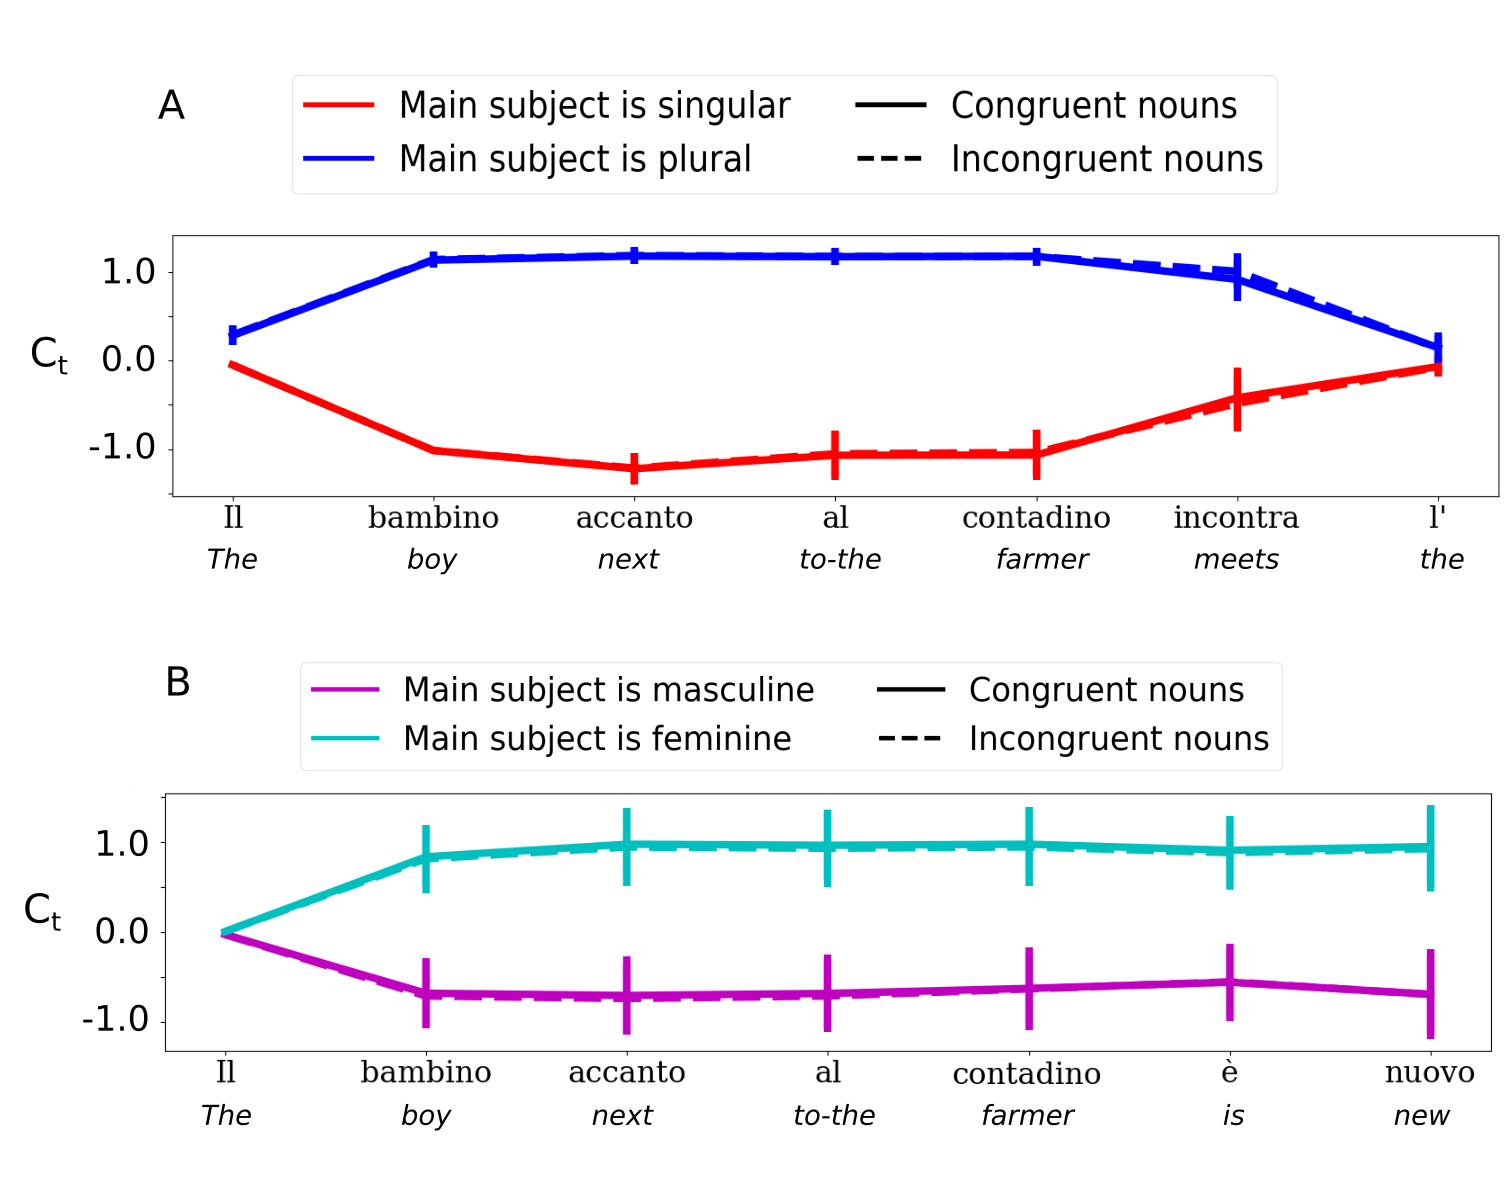
\includegraphics[width=\textwidth]{figures/model_activations_nounpp.png}
    \caption{\textbf{Cell activity of the number unit (panel A) and gender unit (panel B) during the processing of a single long-range dependency across a prepositional phrase:} four conditions are presented, corresponding to whether the main subject of the sentence is singular (red curves) or plural (blue), and to whether the main subject (`bambino') and the intervening noun (`contadino') have the same (congruent) or opposite number (incongruent)}
    \label{fig:nounpp}
\end{figure} 

\subsection{Processing of Two Long-Range Dependencies in the Italian NLM}
Having identified the long-range number unit in the Italian NLM, we now describe its dynamics during the processing of two long-range dependencies. We then describe the error patterns of the Italian NLM on all NA-tasks in the design. As we show, these results confirm that the NLM has an exceptional difficulty to process the embedded verb in Long-Nested:

\subsubsection{The Number Unit Shows Sequential Processing of Two Successive Dependencies and Robust Encoding of the Main Dependency in Nested Constructions}
We first simulated NLM dynamics for all NA-tasks and conditions, by presenting all sentences from each condition to the NLM (methods \ref{}). Figure \ref{fig:2by2_dynamics} presents hidden-state dynamics \YL{replace with cell activation, as in figure 1} of the long-range number unit during the processing of all conditions from the four NA-tasks. We note that, consistent with results on a single dependency, the grammatical number of the main subject is encoded with the same polarity as found in the Noun-PP task - positive for plural (blue) and negative for singular (red). Second, in successive NA-tasks, the activation of the number unit returns to baseline after encountering the main verb ('dice'), and then rises back once the main subject is encountered. This shows that the number unit can sequentially encode two grammatical numbers in two successive dependencies, also in the case in which the two numbers are opposite. In particular, note that in Long-Successive, the grammatical number of the embedded subject is robustly carried across the attractor ('fratello') in the incongruent conditions (dashed lines). Finally, in both Short- and Long-Nested, the grammatical number of the main subject is robustly carried across the main dependency up to the main verb ('evita') \YL{fix xticklabels}, and in particular, across the embedded subject and verb that have an opposite number in some of the conditions (dashed lines).

\begin{figure*}
    \centering
    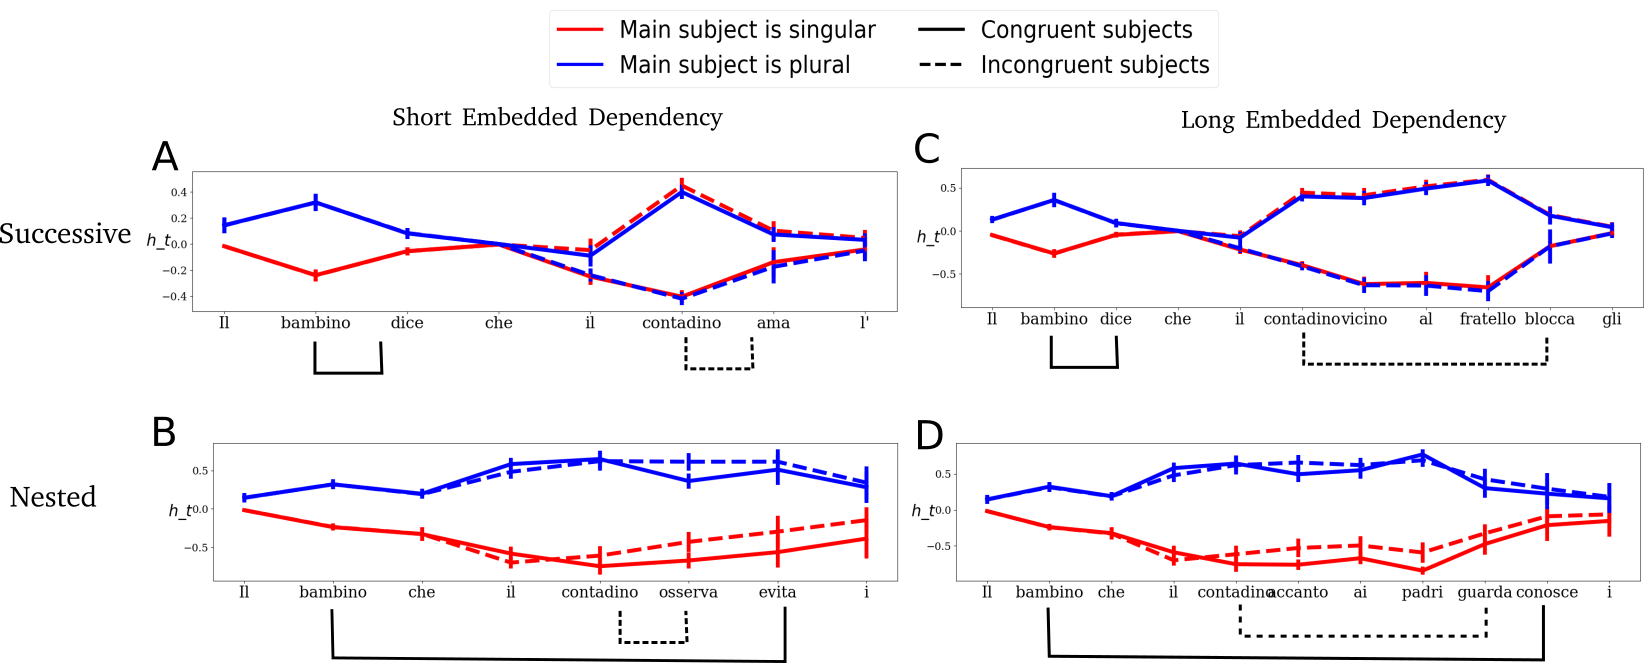
\includegraphics[width=\textwidth]{figures/model_activations.png}
    \caption{\textbf{Dynamics of the hidden activation of the number unit during the processing of two subject-verb dependencies.} Number-unit activity is presented for the four structures in the design: SC-short (panel A), SC-long (B), objRC-short (C) and objRC-long (D). For each structure, results are presented for the four conditions, corresponding to whether the main subject of the sentence is singular (red curves) or plural (blue), and to whether the main and embedded subjects have the same grammatical number (congruent; continuous lines) or not (incongruent; dashed lines).}
    \label{fig:2by2_dynamics}
\end{figure*}


\subsubsection{NLM Performance on Successive Dependencies}
Since no significant processing difficulty is predicted in the successive tasks, we focused our experiments on the embedded agreement, which is expected to be the more difficult one. This has allowed us later to reduce experimental duration with human participants. Also, to facilitate the interpretation of the results, given the relatively large number of conditions, we grouped conditions by whether the main and embedded subjects are congruent (blue) or not (red). Figure \ref{fig:SC_results}A presents the resulting error-rates of the NLM (figure \ref{sm-fig:nested_all_conditions} further provides the full error-rate distribution across all conditions). Several effects are observed in the results: 

\begin{itemize}
    \item \textbf{Near to perfect performance on all conditions}: Overall, for both Short- and Long-Successive, the performance of the NLM was found to be near perfect (\YL{add stats}), with slightly more errors in the Long-Successive case (\YL{add stats}). This is consistent with the sequential encoding observed in the dynamics of the number unit (figure \ref{fig:2by2_dynamics}), which shows a robust encoding of the grammatical number of the embedded subject, also in the presence of an attractor.
    \item \textbf{No subject-congruence effect}: We next tested for a \textit{subject-congruence effect}, i.e., whether incongruent-subject elicited more errors compared to congruent ones. We found no significant subject-congruence effect in neither Short- nor Long-Successive \YL{stats}.
\end{itemize}
 
\subsubsection{NLM Performance on Nested Dependencies}
Figure \ref{fig:objRC_results}A presents the corresponding error-rates in the case of nested dependencies (figure \ref{sm-fig:nested_all_conditions} further provides the full error-rate distribution across all conditions). Several effects are observed in the results:

\begin{itemize}
    \item \textbf{Incongruent conditions elicit more errors}: a significant subject-congruence effect was found on both the embedded and main verbs, in both Short- and Long-Nested (\YL{stats}). In these cases, incongruent subjects elicited more errors compared to congruent subjects.
    \item \textbf{Processing of embedded verbs is more error prone}: for both Short- and Long-Nested, a significant interaction was found between subject-congruence and verb-position, with a larger increase of error rate due to incongruent subjects on the embedded compared to the main verb (\YL{stats}).
    \item \textbf{A longer embedded dependency is more error prone}: for errors made on the embedded verb, we found a significant interaction between subject-congruence and the length of the embedded dependency (Short- vs. Long-Nested), with a larger increase of error-rate due to incongruent subjects in Long-Nested (\YL{stats}).
\end{itemize}
 
\vspace{10pt}

\subsubsection{Discussion of NLM results}
The error-rate patterns of the NLM are overall consistent with the predictions summarized in table \ref{tbl:predictions}: first, successive dependencies are relatively easy for the model, and can be processed sequentially as was confirmed by cell dynamics of the number unit (figure \ref{fig:2by2_dynamics}). Second, the main dependency in both Short- and Long-Nested was successfully processed, although with more overall errors compared to successive dependencies. Third, the NLM made an exceptionally large number of errors on the embedded verb in Long-Nested, as predicted by the sparsity of the long-range mechanism. This was prominent in the case of incongruent-subject, in which the grammatical number of the main subject encoded in the long-range mechanism can interfere. Finally, the NLM made a relatively large number of errors on the embedded verb in Short-Nested, although still significantly above chance level ($error-rate = 0.5$; \YL{stats}). The reduced number of errors in Short- compared to Long-Nested is consistent with the findings about a short-range mechanism that can process the embedded dependency and compensate for the unavailability of the long-range mechanism. 

\YL{refer at some point to the effect of the attractor in SM}.

\subsection{Processing of Two Long-Range Dependencies in Humans}
The previous section has shown that the NLM cannot robustly encode two long-range dependencies that are active at once. The NLM was found to: (1) make an increased error rate on the embedded verb in both Short- and Long-Nested, and (2) to make an exceptionally high error-rate in the latter case, when the embedded dependency was long-range.

Considering the number-agreement mechanism in NLMs as a plausible model for agreement processing in humans, we derive from it the following predictions:

\begin{itemize}
    \item \textbf{Prediction 1}: humans will make more agreement errors on the embedded compared to the main dependency in nested constructions. 
    \item \textbf{Prediction 2}: humans will make more errors on the embedded verb when the embedded dependency is long- compared to short-range. \footnote{\YL{Consider discussing here that regarding Prediction 1, a priori, it could be that an equivalent short-range mechanism in humans would bring the performance on the embedded verb to be comparable, or even better, than that on the main one. So, alternatively, we could also have prediction 1 stated about only the embedded verb in Long-Nested, and prediction 2 as is.}}

\end{itemize}
We tested these predictions by presenting Italian speakers with sentences from the same four NA-tasks in the design (figure \ref{fig:design}; Methods). In what follows, we describe the resulting agreement-error patterns and compare them to those of the NLM.

\subsubsection{Performance on Successive Dependencies}
Figure \ref{fig:SC_results}B presents the resulting error-rates for Short- and Long-Successive. 
\begin{itemize}
    \item \textbf{Relatively low error-rate}: humans made relatively few errors on successive constructions, although significantly above zero (\YL{stats}). Note that in comparison to the Italian NLM, humans have a higher error baseline, to which unrelated factors that are specific to humans may contribute, such as occasional lapses of attention.
    \item \textbf{Weak subject-congruence effect}: we found no significant subject-congruence effect in Short-Successive, and a marginally significant subject-congruence effect in Long-Successive (\YL{stats}).
\end{itemize}
\YL{compare also to performance on noun-PP}.

\subsubsection{Performance on Nested Dependencies}
Figure \ref{fig:objRC_results}B presents errors-rate for the Short- and Long-Nested. Several effects are observed in the results: 
\begin{itemize}
    \item \textbf{Subject-congruence effect on embedded verbs}: for the embedded verb in both Short- and Long-Nested, incongurent subject elicited more errors - a significant subject-congruence effect was found in both cases \YL{stats}
    \item \textbf{No subject-congruence on main verb}: in contrast, for the main verb, no subject-congruence effect was found, in neither Short- nor Long-Nested. \YL{stats}
    \item \textbf{Processing of embedded verbs is more error prone}: for both Short- and Long-Nested, the increase in error rate due to incongruent subjects was larger for embedded compared to main verbs - a significant interaction was found between subject congruence and verb position in both cases \YL{stats}.
    \item \textbf{A longer embedded dependency is more error prone}: for embedded verbs, the increase in error-rate due to incongruent subjects was comparable when the embedded long-range dependency was long compared to short - no significant interaction was found between subject-congruence and length of the embedded dependency (Short- vs. Long-Nested). However, crucially, this interaction was found significant when the main subject was plural (figure S4). \YL{Consider nonetheless to present in the main text only the results for plural main subject and put in SM the collated results. It seems justified given the results in previous studies.}
\end{itemize}

    

  
\subsubsection{Discussion of human results}
Overall, successive dependencies were, as expected, relatively easy for humans compared to nested. Subject-congruence effect was not found, or was marginally significant, which is consistent with sequential processing of grammatical number as was found in NLMs. The results confirm \textit{Prediction 1} - the main dependency in both Short- and Long-Nested was processed more robustly than the embedded one, as was confirmed by a significant interaction between subject-congruence and verb position. Finally, the results confirm \textit{Prediction 2} - the embedded dependency was more difficult to process when it was long range, as was confirmed by a significant interaction between subject-congruence and the length of the embedded dependency. This effect was significant only when the main subject was plural, which is in accordance with the well-established effect of number marking on agreement errors, reported in both production (\citet{Bock:Miller:1991, bock1993meaning, eberhard1997marked}; for Italian, see, \citet{vigliocco1995constructing}) and comprehension \citep[e.g.,][]{pearlmutter1999agreement, wagers2009agreement, lago2015agreement}. In these studies, participants made more errors when the head noun was singular and the attractor plural. Specifically, in comprehension, \citet{wagers2009agreement} showed that processing facilitation of an embedded dependency in ungrammatical sentences occurred when the attractor (the main subject in this case) was plural.

\vspace{10pt}
Taken together, the results from the experiments show that there are key points of similarities between the agreement-error patterns produced by humans and NLMs. \ref{tbl:comparison} summarizes and compares these effects. As can be seen in the table, most of the key effects were found in both humans and NLMs. The main point of discrepancy regards subject-congruence effect on the main verb in nested constructions, which was found only for RNNs. We return to this point in the General Discussion, when we discuss interference dynamics in the model.

\begin{table}[h]
\tiny
\centering
\parbox{.4\linewidth}{
\centering
    \begin{tabular}{ |P{3cm}|P{1.3cm}|P{1.3cm}|  }
    \hline
    \rowcolor{cyan}
    \multicolumn{3}{|c|}{\textbf{Short-Successive}} \\
    \hline
    \rowcolor{cyan}
    \textbf{Effect} & \textbf{Humans} & \textbf{RNNs} \\
    \Xhline{3\arrayrulewidth}
    \rowcolor{green}
    \textbf{Subject Congruence (Embedded verb)} & X & X \\
    \hline
    
    \end{tabular}
}
\hfill
\parbox{.4\linewidth}{
\centering
    \begin{tabular}{ |P{3cm}|P{1.3cm}|P{1.3cm}|  }
    \hline
    \rowcolor{cyan}
    \multicolumn{3}{|c|}{\textbf{Long-Successive}} \\
    \hline
    \rowcolor{cyan}
    \textbf{Effect} & \textbf{Humans} & \textbf{RNNs} \\
    \Xhline{3\arrayrulewidth}
    \rowcolor{green}
    \textbf{Subject Congruence (Embedded verb)} & X & X \\
    \hline
    
    \end{tabular}
}

\vspace{25pt}

\parbox{.4\linewidth}{
\centering
    \begin{tabular}{ |P{3cm}|P{1.3cm}|P{1.3cm}|  }
    \hline
    \rowcolor{cyan}
    \multicolumn{3}{|c|}{\textbf{Short-Nested}} \\
    \hline
    \rowcolor{cyan}
    \textbf{Effect} & \textbf{Humans} & \textbf{RNNs} \\
    \Xhline{3\arrayrulewidth}
    \rowcolor{magenta}
    \textbf{Subject Congruence (Main verb)} & X &  V\\
    \Xhline{3\arrayrulewidth}
    \rowcolor{green}
    \textbf{Subject Congruence (Embedded verb)} & V &  V\\
    \hline
    \rowcolor{green}
    \textbf{Interaction: Subject-Congruence Verb-Position} & V &  V\\
    \hline
    
    \end{tabular}
}
\hfill
\parbox{.4\linewidth}{
\centering
    \begin{tabular}{ |P{3cm}|P{1.3cm}|P{1.3cm}|  }
    \hline
    \rowcolor{cyan}
    \multicolumn{3}{|c|}{\textbf{Long-Nested}} \\
    \hline
    \rowcolor{cyan}
    \textbf{Effect} & \textbf{Humans} & \textbf{RNNs} \\
    \Xhline{3\arrayrulewidth}
    \rowcolor{magenta}
    \textbf{Subject Congruence (Main verb)} & X &  V\\
    \Xhline{3\arrayrulewidth}
    \rowcolor{green}
    \textbf{Subject Congruence (Embedded verb)} & V &  V\\
    \hline
    \rowcolor{green}
    \textbf{Interaction: Subject-Congruence Verb-Position} & V &  V\\
    \hline
    
    \end{tabular}
}
\caption{A summary of all effects  humans and RNNs.}
\label{tbl:comparison}
\end{table}



\begin{figure*}[h]
    \centering
    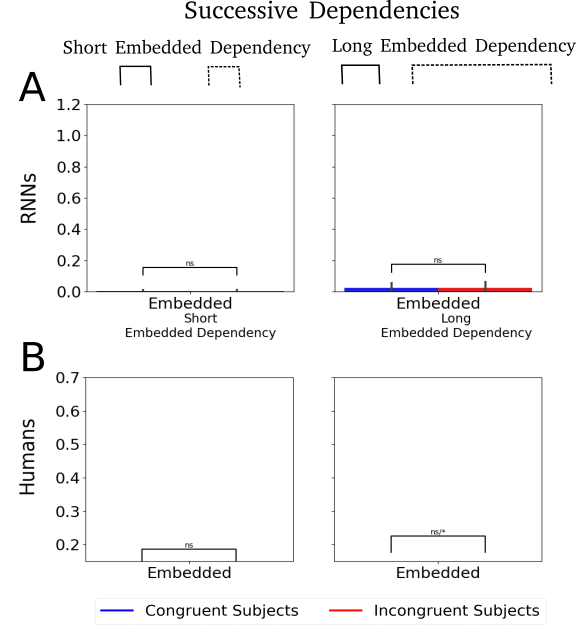
\includegraphics[width=10cm]{figures/error_rates_successive.png}
    \caption{\textbf{Error rates on the SC-short and SC-long structures:} collected from NLMs (panel A) and human subjects (B). Blue and red bars correspond to whether the main and embedded subjects agree on number (congruent subjects) or not (incongruent), respectively). Error bars represent standard error of the mean across all trials. ns - non significant.}
    \label{fig:SC_results}
\end{figure*}


\begin{figure*}[h]
    \centering
    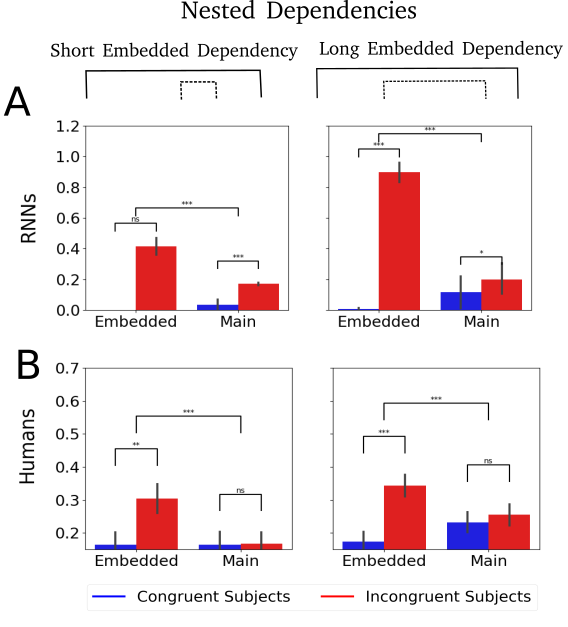
\includegraphics[width=10cm]{figures/error_rates_nested.png}
    \caption{\textbf{Error rates on the objRC-short and objRC-long structures:} collected from NLMs (panel A) and humans subjects (panel B). Blue and red bars correspond to whether the main and embedded subjects agree on number (congruent subjects) or not (incongruent), respectively. Error bars represent standard error of the mean across all trials. ns - non significant.}
    \label{fig:objRC_results}
\end{figure*}

 
% \YL{discuss marked case and the corresponding results.}

